\documentclass[review]{elsarticle} %review=doublespace preprint=single 5p=2 column
%%% Begin My package additions %%%%%%%%%%%%%%%%%%%
\usepackage[hyphens]{url}



\usepackage{lineno} % add
  \linenumbers % turns line numbering on
\providecommand{\tightlist}{%
  \setlength{\itemsep}{0pt}\setlength{\parskip}{0pt}}

\usepackage{graphicx}
\usepackage{booktabs} % book-quality tables
%%%%%%%%%%%%%%%% end my additions to header

\usepackage[T1]{fontenc}
\usepackage{lmodern}
\usepackage{amssymb,amsmath}
\usepackage{ifxetex,ifluatex}
\usepackage{fixltx2e} % provides \textsubscript
% use upquote if available, for straight quotes in verbatim environments
\IfFileExists{upquote.sty}{\usepackage{upquote}}{}
\ifnum 0\ifxetex 1\fi\ifluatex 1\fi=0 % if pdftex
  \usepackage[utf8]{inputenc}
\else % if luatex or xelatex
  \usepackage{fontspec}
  \ifxetex
    \usepackage{xltxtra,xunicode}
  \fi
  \defaultfontfeatures{Mapping=tex-text,Scale=MatchLowercase}
  \newcommand{\euro}{€}
\fi
% use microtype if available
\IfFileExists{microtype.sty}{\usepackage{microtype}}{}
\bibliographystyle{elsarticle-harv}
\usepackage{color}
\usepackage{fancyvrb}
\newcommand{\VerbBar}{|}
\newcommand{\VERB}{\Verb[commandchars=\\\{\}]}
\DefineVerbatimEnvironment{Highlighting}{Verbatim}{commandchars=\\\{\}}
% Add ',fontsize=\small' for more characters per line
\usepackage{framed}
\definecolor{shadecolor}{RGB}{248,248,248}
\newenvironment{Shaded}{\begin{snugshade}}{\end{snugshade}}
\newcommand{\AlertTok}[1]{\textcolor[rgb]{0.94,0.16,0.16}{#1}}
\newcommand{\AnnotationTok}[1]{\textcolor[rgb]{0.56,0.35,0.01}{\textbf{\textit{#1}}}}
\newcommand{\AttributeTok}[1]{\textcolor[rgb]{0.77,0.63,0.00}{#1}}
\newcommand{\BaseNTok}[1]{\textcolor[rgb]{0.00,0.00,0.81}{#1}}
\newcommand{\BuiltInTok}[1]{#1}
\newcommand{\CharTok}[1]{\textcolor[rgb]{0.31,0.60,0.02}{#1}}
\newcommand{\CommentTok}[1]{\textcolor[rgb]{0.56,0.35,0.01}{\textit{#1}}}
\newcommand{\CommentVarTok}[1]{\textcolor[rgb]{0.56,0.35,0.01}{\textbf{\textit{#1}}}}
\newcommand{\ConstantTok}[1]{\textcolor[rgb]{0.00,0.00,0.00}{#1}}
\newcommand{\ControlFlowTok}[1]{\textcolor[rgb]{0.13,0.29,0.53}{\textbf{#1}}}
\newcommand{\DataTypeTok}[1]{\textcolor[rgb]{0.13,0.29,0.53}{#1}}
\newcommand{\DecValTok}[1]{\textcolor[rgb]{0.00,0.00,0.81}{#1}}
\newcommand{\DocumentationTok}[1]{\textcolor[rgb]{0.56,0.35,0.01}{\textbf{\textit{#1}}}}
\newcommand{\ErrorTok}[1]{\textcolor[rgb]{0.64,0.00,0.00}{\textbf{#1}}}
\newcommand{\ExtensionTok}[1]{#1}
\newcommand{\FloatTok}[1]{\textcolor[rgb]{0.00,0.00,0.81}{#1}}
\newcommand{\FunctionTok}[1]{\textcolor[rgb]{0.00,0.00,0.00}{#1}}
\newcommand{\ImportTok}[1]{#1}
\newcommand{\InformationTok}[1]{\textcolor[rgb]{0.56,0.35,0.01}{\textbf{\textit{#1}}}}
\newcommand{\KeywordTok}[1]{\textcolor[rgb]{0.13,0.29,0.53}{\textbf{#1}}}
\newcommand{\NormalTok}[1]{#1}
\newcommand{\OperatorTok}[1]{\textcolor[rgb]{0.81,0.36,0.00}{\textbf{#1}}}
\newcommand{\OtherTok}[1]{\textcolor[rgb]{0.56,0.35,0.01}{#1}}
\newcommand{\PreprocessorTok}[1]{\textcolor[rgb]{0.56,0.35,0.01}{\textit{#1}}}
\newcommand{\RegionMarkerTok}[1]{#1}
\newcommand{\SpecialCharTok}[1]{\textcolor[rgb]{0.00,0.00,0.00}{#1}}
\newcommand{\SpecialStringTok}[1]{\textcolor[rgb]{0.31,0.60,0.02}{#1}}
\newcommand{\StringTok}[1]{\textcolor[rgb]{0.31,0.60,0.02}{#1}}
\newcommand{\VariableTok}[1]{\textcolor[rgb]{0.00,0.00,0.00}{#1}}
\newcommand{\VerbatimStringTok}[1]{\textcolor[rgb]{0.31,0.60,0.02}{#1}}
\newcommand{\WarningTok}[1]{\textcolor[rgb]{0.56,0.35,0.01}{\textbf{\textit{#1}}}}
\usepackage{longtable}
\usepackage{graphicx}
% We will generate all images so they have a width \maxwidth. This means
% that they will get their normal width if they fit onto the page, but
% are scaled down if they would overflow the margins.
\makeatletter
\def\maxwidth{\ifdim\Gin@nat@width>\linewidth\linewidth
\else\Gin@nat@width\fi}
\makeatother
\let\Oldincludegraphics\includegraphics
\renewcommand{\includegraphics}[1]{\Oldincludegraphics[width=\maxwidth]{#1}}
\ifxetex
  \usepackage[setpagesize=false, % page size defined by xetex
              unicode=false, % unicode breaks when used with xetex
              xetex]{hyperref}
\else
  \usepackage[unicode=true]{hyperref}
\fi
\hypersetup{breaklinks=true,
            bookmarks=true,
            pdfauthor={},
            pdftitle={dfoliatR: An R package for detection and analysis of insect defoliation signals in tree rings},
            colorlinks=false,
            urlcolor=blue,
            linkcolor=magenta,
            pdfborder={0 0 0}}
\urlstyle{same}  % don't use monospace font for urls

\setcounter{secnumdepth}{5}
% Pandoc toggle for numbering sections (defaults to be off)


% Pandoc header
\usepackage{booktabs}
\usepackage{longtable}
\usepackage{array}
\usepackage{multirow}
\usepackage{wrapfig}
\usepackage{float}
\usepackage{colortbl}
\usepackage{pdflscape}
\usepackage{tabu}
\usepackage{threeparttable}
\usepackage{threeparttablex}
\usepackage[normalem]{ulem}
\usepackage{makecell}
\usepackage{xcolor}

\usepackage{amsmath}
\usepackage{float}
\usepackage{booktabs}
\makeatletter
\def\ps@pprintTitle{%
 \let\@oddhead\@empty
 \let\@evenhead\@empty
 \let\@oddfoot\@empty
 \let\@evenfoot\@oddfoot
}
\makeatother

\begin{document}
\begin{frontmatter}

  \title{\texttt{dfoliatR}: An R package for detection and analysis of insect defoliation signals in tree rings}
    \author[a,b]{Christopher H. Guiterman\corref{1}}
   \ead{chguiterman@arizona.edu} 
    \author[a,c]{Ann M. Lynch}
   \ead{ann.m.lynch@usda.gov} 
    \author[d]{Jodi N. Axelson}
   \ead{jodi.axelson@berkeley.edu} 
      \address[a]{Laboratory of Tree-Ring Research, University of Arizona, 1215 E Lowell St.~Box 210045, Tucson, AZ, 85721}
    \address[b]{Three Pines Forest Research, LLC, PO Box 225, Etna, NH, 03750}
    \address[c]{U.S. Forest Service, Rocky Mountain Research Station, 1215 E Lowell St.~Box 210045, Tucson, AZ, 85721}
    \address[d]{Dept of Environmental Science, Policy \& Management, University of California, Berkeley, 130 Mulford Hall \#3114, Berkeley, CA 94720}
      \cortext[1]{Corresponding Author}
  
  \begin{abstract}
  We present a new \texttt{R} package to provide dendroecologists with tools to infer, quantify, analyze, and visualize growth suppression events in tree rings. \texttt{dfoliatR} is based on the OUTBREAK program and builds on existing resources in the \texttt{R} computing environment and the well-used \texttt{dplR} package. It is designed to aid research in the ecology of insect defoliation events and to reconstruct defoliator outbreak chronologies, but can be applied to other studies where host--non-host comparisons are useful. \texttt{dfoliatR} performs an indexing procedure to remove climatic signals in the host-tree series that are represented in the non-host chronology, or other annually-resolved climate series. It then infers defoliation events in individual trees based on user-specified thresholds. Site-level analyses identify outbreak events that synchronously affect user-defined numbers or proportions of involved host trees. Functions are provided for summary statistics and graphics of tree- and site-level series. We evaluated \texttt{dfoliatR} against OUTBREAK, using eight datasets including 222 host-trees, and found that \texttt{dfoliatR} improves on OUTBREAK with greater user control, identification of defoliation events, computing capacity, and both the statistical summary and graphical outputs. We provide two example data sets and script to enable users to gain familiarity with the package and its capabilities. The source code is available in the Comprehensive R Archive Network (CRAN) and on GitHub.
  \end{abstract}
   \begin{keyword} Dendroecology, dendroentomology, OUTBREAK, western spruce budworm, defoliator regimes, insect outbreak reconstruction\end{keyword}
 \end{frontmatter}

\begin{quote}
This article is published as: Guiterman, CH, AM Lynch, and JN Axelson (2020) \texttt{dfoliatR}: An R package for detection and analysis of insect defoliation signals in tree rings. \emph{Dendrochronologia}. DOI: 10.1016/j.dendro.2020.125750. Available for free \href{https://authors.elsevier.com/sd/article/S1125786520300898}{(link)}
\end{quote}

\hypertarget{introduction}{%
\section{Introduction}\label{introduction}}

Variation in the width and morphology of annual radial growth rings in trees permits dating and quantification of past forest insect defoliator outbreaks. Defoliation can be distinguished from climate- and other disturbance-related influences by comparing ring-width or other annually-resolved features in the wood of host species to that of non-host species or annually-resolved climate records. The effect of defoliation on radial growth of trees has been recognized since the 1860s, and used to reconstruct outbreak regimes since the 1950s (Blais, 1954; Alfaro et al., 1982; Lynch, 2012). It was not until the 1980s, however, that precise dendrochronological techniques were applied for inferring defoliation events and reconstructing defoliator outbreak regimes (Swetnam et al., 1985; Speer, 2010; Lynch, 2012). The first studies (Swetnam et al., 1985; Swetnam and Lynch, 1989, 1993) focused on developing historical outbreak reconstructions of western spruce budworm (WSBW; \emph{Choristoneura freemani} (Lepidoptera: Tortricidae); previously known as \emph{C. occidentalis}). The methodology has since been successfully applied to a wide range of defoliator species, most of which are conifer herbivores, and has evolved in sophistication for a wide range of ecosystem situations (Lynch, 2012).

The main dendrochronological tool for inferring, dating, and characterizing defoliator outbreaks from tree-ring records has been the software routine OUTBREAK (Swetnam et al., 1985; Holmes and Swetnam, 1986; Swetnam and Lynch, 1989). OUTBREAK computes indices (described later in detail) of suppressed growth by subtracting a detrended and standardized climate series (a ``control'' chronology) from individual host-tree detrended and standardized radial growth series after the host and non-host series have been brought to a common variance. The non-host chronology usually consists of a site chronology developed from non-host tree species growing on a climate-sensitive site, but a gridded climate data point series, like the North American Drought Atlas (Cook and Krusic, 2004) also suffices. If the host and non-host species respond similarly to climate (which can and should be tested), the derived series retains variability that the host and non-host series do not have in common, generally the insect signal and some unexplained variability (noise). The user defines a rule base specifying the magnitude and duration that a period of indexed growth suppression must meet or surpass for a period of suppressed growth to be inferred as a defoliation event at the tree level. Rule bases are derived from the user's knowledge of insect and host ecologies, and from consideration of the likelihood and relative importance of Type I and II errors.

Though powerful, OUTBREAK is outdated and increasingly difficult to use in modern computing environments. It was written in FORTRAN V with inherently severe restrictions, as RAM and disk space were limited at that time (256 kb and 10 MB, respectively) and FORTRAN conventions imposed very strict formatting, file naming, and output conventions. The program lacks a graphical interface or capabilities, forcing users to import generated text files into spreadsheets or other software to assess results and perform analyses. Furthermore, OUTBREAK can only handle one test at a time, creating barriers to batch operation and a large burden for researchers with datasets including multiple sites. We developed \texttt{dfoliatR} (Guiterman et al., 2020) as an \texttt{R}- and \texttt{dplR}-based library to overcome these issues.

\texttt{dfoliatR} adds to a growing suite of dendrochronology packages in the \texttt{R} computing environment (R Core Team, 2019). Stemming from the \texttt{dplR} library (Bunn, 2008) that enables \texttt{R} users to read and write an array of tree-ring data formats, standardize ring width series, build and evaluate chronologies, and perform quality control (to name a few), one can now also measure ring widths from scanned images of prepared samples (Lara et al., 2015; Shi et al., 2019), conduct and check crossdating (Bunn, 2010), analyze sub-annual anatomical features (Rathgeber et al., 2011; Campelo et al., 2016), and perform many analytical tests (Zang and Biondi, 2015; Jevšenak and Levanič, 2018). Tools for assessing stand dynamics and disturbance analyses are under rapid development, with new packages for assessing release events (\texttt{TRADER}: Altman et al., 2014), metrics of growth resilience (\texttt{pointRes}: van der Maaten-Theunissen et al., 2015), and fire history (\texttt{burnr}: Malevich et al., 2018). The key objective of \texttt{dfoliatR} is to provide tools to identify and analyze insect defoliation and outbreak events by building on the methods employed by OUTBREAK. It capitalizes on the robust software already available in \texttt{R} by using \texttt{dplR} data formats for incoming tree-ring series and providing output data formats embodied by the \texttt{tidyverse} (Wickham et al., 2019) that include efficient data manipulation (\texttt{dplyr}: Wickham et al., 2020) and graphics (\texttt{ggplot2}: Wickham, 2016).

In this paper, we describe the statistical methods employed by \texttt{dfoliatR}, compare results to those produced by OUTBREAK, and present an example analysis including test data sets and script. Users need not have much experience in \texttt{R} to replicate the analyses and graphics as presented. The \texttt{R} code below is executable in an \texttt{R} session once the required libraries are installed and loaded. Support documentation in addition to this paper is provided within the package via standard help menus and on the package website (\url{https://chguiterman.github.io/dfoliatR/}), which includes up-to-date vignettes that describe various routines. Code to generate a preprint of this manuscript, including the \texttt{R} scripts and tabular and graphical output is available from \url{https://github.com/chguiterman/dfoliatR_paper}.

\hypertarget{overview-of-the-software}{%
\section{Overview of the software}\label{overview-of-the-software}}

The \texttt{dfoliatR} library requires two sets of tree-ring data to infer defoliation and outbreak events:

\begin{itemize}
\tightlist
\item
  Standardized ring-width series for individual trees of the host species
\item
  A standardized tree-ring chronology from a local non-host species, or a climate reconstruction
\end{itemize}

Users can develop these data sets in the software of their choosing, such as \texttt{dplR} or ARSTAN (Cook and Holmes, 1996). It is important that the host-tree data include only one tree-ring series per tree. \texttt{dplR} (via the \texttt{dplR::treeMean()} function) and dpl versions of ARSTAN have options for averaging multiple sample series into a tree-level series.

At the heart of \texttt{dfoliatR} lies two functions: \texttt{defoliate\_trees()} and \texttt{outbreak()}. These identify defoliation events on individual trees (Figure \ref{fig:fig-defol}) and then composite across multiple trees to infer stand or site level outbreak events (Figure \ref{fig:fig-obr}).



\begin{figure}
\centering
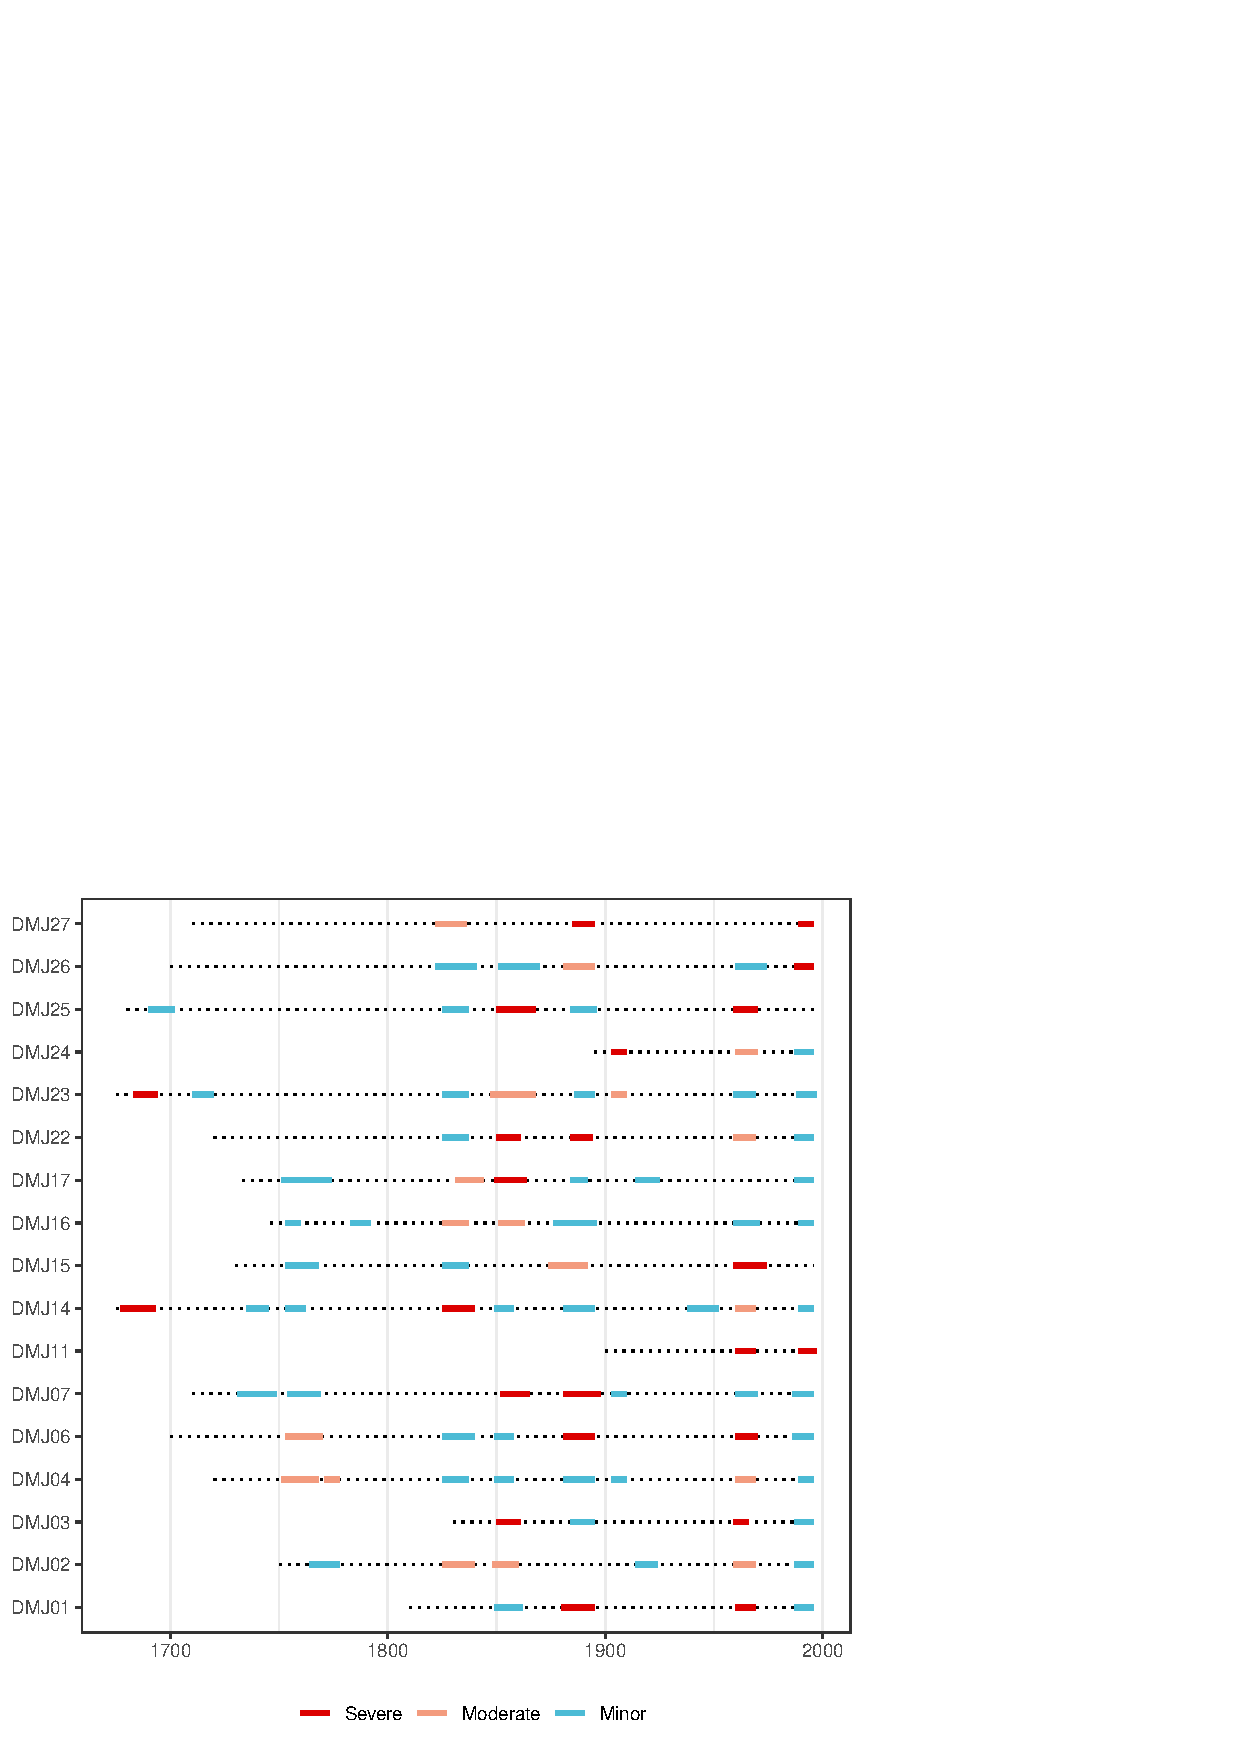
\includegraphics{D:/Dropbox/dfoliatR_paper/Output/tree-plot-default.pdf}
\caption{\label{fig:fig-defol}Default \texttt{dfoliatR} graphic for individual trees, produced by the \texttt{plot\_defol()} function. The series names from the DMJ site (Ryerson et al., 2003) are listed on the Y-axis, dotted lines represent the series length for each tree, and colored segments show periods of defoliation. The colors of defoliation segments represent its severity, for which users can define cut-off values to determine severe--moderate--minor defoliation intensities. The default break points for severity classes are the mean and first quartile for event NGSI values. Colors and other features of the graphic can be adjusted using \texttt{ggplot2} parameters, as shown below.}
\end{figure}



\begin{figure}
\centering
\includegraphics{D:/Dropbox/dfoliatR_paper/Output/site-plot.pdf}
\caption{\label{fig:fig-obr}Default \texttt{dfoliatR} graphic for site-level outbreak events, produced by the \texttt{plot\_outbreak()} function. These plots summarize the data in Figure \ref{fig:fig-defol} for the DMJ site. Top panel shows the sample depth, the middle panel shows the mean GSI with inferred outbreak events filled, and the bottom panel shows the percent of trees defoliated, used to identify time periods of inferred outbreaks.}
\end{figure}

\hypertarget{identifying-defoliation-of-trees}{%
\subsection{Identifying Defoliation of Trees}\label{identifying-defoliation-of-trees}}

The \texttt{defoliate\_trees()} function is the point of entry to the \texttt{dfoliatR} library. It performs two processes, removing climate-related growth signals from the host-tree series and identifying tree-level defoliation events. The climatic or non-defoliation signals in each host-tree series are characterized by a non-host chronology or climate reconstruction. \texttt{dfoliatR} removes the non-defoliation signal by subtracting the non-host series from each host-tree series, which generates a residual index. In OUTBREAK, this residual index was termed the ``corrected index.'' We call it the ``growth suppression index'' (GSI). The GSI is calculated the same as in OUTBREAK for each host tree as
\begin{align}
\textrm{GSI}_{i} = \textrm{H}_{i} - \left( \textrm{NH}_{i} - \overline{\textrm{NH}} \right) \frac{\sigma_{\textrm{H}}}{\sigma_{\textrm{NH}}} \
\end{align}
where H and NH are the host-tree series and the non-host chronology, in year i, respectively. Only the common period between the host-tree series and the non-host chronology are used in Equation 1. The host and non-host chronologies are brought to common variance by scaling the non-host chronology by its mean (\(\overline{\textrm{NH}}\)) and multiplying by the ratio of host and non-host standard deviations (\(\frac{\sigma_{\textrm{H}}}{\sigma_{\textrm{NH}}}\)), which approximates the variance of the host tree series.

Negative departures in the normalized GSI (NGSI, or GSI converted to z-scores) that surpass user-specified thresholds in duration and magnitude are defined as \emph{defoliation events}. As in OUTBREAK, the lowest NGSI value in the particular sequence being assessed must reach the magnitude threshold. The default setting is -1.28 (NGSI is in units of standard deviation), which was previously determined to be representative of WSBW effects (Swetnam and Lynch, 1989) and is commonly used for other species (see Lynch, 2012). The year with the lowest value is termed the ``year of maximum departure'' and becomes a central point in time for assessing other thresholds before being included as a defoliation event. If the year of maximum departure is higher than the threshold (i.e.~\(\textrm{NGSI}_{lowest} > -1.28\)), the sequence being assessed is omitted from the event results.

Event duration is assessed by examining sequences of negative NGSI (for which one or more values exceeded the magnitude threshold) before and after the year of maximum departure. Each defoliation event is allowed one single-year positive excursion on each side of the year of maximum departure. Duration is computed across the entire sequence that may include these two positive excursions. As in OUTBREAK, the user specifies a duration threshold (minimum number of years) for a departure sequence to be inferred as a defoliation event. The default threshold is eight years, as is commonly used in WSBW studies (Swetnam and Lynch, 1989). If the sequence is shorter than the duration threshold, the sequence is omitted from the event results (i.e., both thresholds must be met). Researchers can, and should, adjust the duration and magnitude parameters accordingly and critically evaluate the results, as insect species vary in the length of their outbreaks and the degree to which they can suppress tree growth. OUTBREAK provides two sets of default values, those for WSBW, which typically has lengthy outbreaks, and ones for Douglas-fir tussock moth (\emph{Orgyia pseudotsugata} (Lepidoptera: Tortricidae)) of three years duration with -1.28 departure threshold that may be suitable for more eruptive species.

Like OUTBREAK, users are provided an option to suspend the duration threshold at the recent end of the series in cases where an outbreak event is known to be ongoing. This should be used if the user has direct knowledge of defoliation at the site during the sampling campaign. The advantage of allowing potentially short, series-end events is that it allows a current event to be included in return-interval estimates, and can aid in identifying the start-year for the current defoliation event or outbreak.

Diverging from OUTBREAK, \texttt{dfoliatR} includes an option allowing users to extend defoliation events on individual trees by bridging between sequential events (Figure \ref{fig:fig-bridge}). In cases where two defoliation events are separated by a single year, bridging will link them into a single event. This option was added to \texttt{dfoliatR} during the testing phase of development, when we realized that OUTBREAK deliberately omits sequential, or back-to-back events, even when both events surpass the magnitude and duration thresholds. Instead, OUTBREAK will select the one sequential event with the lowest negative departure year. In every case we assessed (described below) we felt that the OUTBREAK-omitted defoliation events should have been maintained and recorded. Due in large part to reconstructions using OUTBREAK (see papers cited by Lynch, 2012), we now know considerably more about forest defoliator outbreak regimes than we did in the 1980s when OUTBREAK was under development. We think that two or more prolonged events separated by a single year should in some situations be considered a single event. This is particularly relevant to WSBW and spruce budworm (\emph{C. fumiferana}), for which multiple outbreak regime reconstruction, as well as other research and forest health observations, show that outbreaks can be very long (Schmitt et al., 1984; Sanders et al., 1985; Brookes et al., 1987, and many later publications). Often the greatest growth suppression occurs late in the outbreak due to lag effects between defoliation and radial growth, and to cumulative effects accrued on a tree's resources (Brubaker, 1978; Alfaro et al., 1982; Wickman, 1986; Swetnam and Lynch, 1989, 1993; Mason et al., 1997; Axelson et al., 2014). We urge caution in using the bridging option, however, because it may not be appropriate for all studied insects, such as in situations where impacted stands barely recover from one outbreak before another begins, as with pine processionary caterpillars (\emph{Thaumetopoea pityocampa} (Lepidoptera: Thaumetopoeidae)) (Carus, 2004, 2009) or where outbreaks are known to be very short, such as larch budmoth (\emph{Zeiraphera diniana} Gn.) in the European Alps (Esper et al., 2007).



\begin{figure}
\centering
\includegraphics{D:/Dropbox/dfoliatR_paper/Output/bridging_color.pdf}
\caption{\label{fig:fig-bridge}Examples of identified defoliation events on individual trees. For each tree (DMJ26 and EFK22), OUTBREAK and \texttt{dfoliatR} identify most of the same events, but there is one added event (in blue) that was omitted by OUTBREAK. These were omitted because they were separated by a single year of positive normalized growth suppression index (NGSI) and OUTBREAK selected the one event with the lowest maximum departure value. \texttt{dfoliatR} provides an option to bridge these sequential events into single long events that may better represent the duration of defoliation given the insect and sites under consideration.}
\end{figure}

\hypertarget{inferring-outbreak-events}{%
\subsection{Inferring Outbreak Events}\label{inferring-outbreak-events}}

Defoliation of one or a few trees does not constitute an outbreak. To determine when defoliation becomes an \emph{outbreak event}, \texttt{dfoliatR} composites the individual tree defoliation series into a site-level chronology with the \texttt{outbreak()} function. Users have options to define the number and/or the proportion of trees required for an event to be considered an outbreak. Three parameters control whether a defoliation event constitutes an outbreak: the minimum number of trees available, the minimum number of trees recording defoliation, and the percent of trees recording defoliation. The first allows the researcher to make a judgment call as to the confidence ascribed to reduced sample depth toward the ends of their chronologies, thus compensating for the ``fading record problem'' (Swetnam et al., 1999). The second two parameters adjust the scale of defoliation considered to be an outbreak. Absolute numbers of trees and percentages can be applied separately or in conjunction, following filtering conventions in tree-ring fire history studies (Malevich et al., 2018). We urge users to carefully consider the choice of absolute numbers in situations where the number of trees represented in the series varies with time, or the choice of percentages when sample size is small.

\hypertarget{evaluation}{%
\section{Evaluation}\label{evaluation}}

\hypertarget{approach}{%
\subsection{Approach}\label{approach}}

We tested \texttt{dfoliatR} against OUTBREAK by comparing NGSI to OUTBREAK's normalized corrected indices for individual trees and years, defoliation status for individual trees and years, and percentage of trees recording outbreaks at the site level. Our tests used standardized ring-width data from eight host-tree sites spanning the range of WSBW. The sites were sampled in British Columbia (Axelson et al., 2015), Wyoming (Axelson et al., 2018), Colorado (Ryerson et al., 2003), and New Mexico (Swetnam and Lynch, 1993). These host data were compared to non-host chronologies from the original studies, but we made no effort here to replicate the reconstructions or analyses of those studies.

We detrended host data for both \texttt{dfoliatR} and OUTBREAK using ARSTAN (version 6.1) with cubic smoothing splines (50\% frequency response on 100-150 year wavelengths depending on the site). In both \texttt{dfoliatR} and OUTBREAK we used event thresholds of -1.28 normalized indices, 8 years duration, and allowed for events at the end of series in seven of eight sites that had known outbreaks at the time of sampling. We found it necessary to be consistent in how we detrended and what software we employed (e.g., ARSTAN vs \texttt{dplR}) because subtle differences in standardized ring-width indices generated between the programs transferred into differences between \texttt{dfoliatR} and OUTBREAK. In the end, we chose to only use the standardization output files from ARSTAN, which are easily read into \texttt{R} (and then \texttt{dfoliatR}) using the \texttt{dplR} package.

The \texttt{R} code to replicate our comparisons is available from \url{https://github.com/chguiterman/dfoliatR_paper}.

\hypertarget{findings}{%
\subsection{Findings}\label{findings}}

Across the 43,280 ring-width indices from 222 trees included in our evaluation, we found that \texttt{dfoliatR} and OUTBREAK compute identical growth suppression indices at 0.00 precision. We expected this outcome because both programs apply Equation 1 to calcuate disturbance indices. At the tree-level, the programs identified 11,530 total index years with defoliation. The programs agreed on 97.9\% of the years, leaving 927 ``difference'' years in which only one program identified defoliation on an individual tree. The differences included 102 events on 85 trees. We carefully inspected each of these events in the full context of each tree's ring-series, and categorized the differences as follows

\begin{itemize}
\item
  \emph{Series-end events} (40\% of the total) in which OUTBREAK included ``truncated outbreaks'' (for seven sites) at the end of each series. In \texttt{dfoliatR}, this option is controlled by the ``series\_end\_events'' parameter to \texttt{defoliate\_trees()}. In OUTBREAK, the option appears while changing the duration parameter (option 3). When selected, OUTBREAK will include any sequences of negative indices at the beginning and the end of each tree series as a defoliation event, without consideration of either duration or magnitude thresholds. In \texttt{dfoliatR}, the duration threshold is omitted and the magnitude threshold is retained in series-end-events. Each of the 13 events included in these differences did not meet the ``max\_reduction'' parameter (-1.28 NGSI) in \texttt{dfoliatR} and were excluded. In two cases, OUTBREAK included events at the beginning of the series where \texttt{dfoliatR} does not allow truncated events. In four cases, OUTBREAK omitted only the last year of the series because the index was positive, but \texttt{dfoliatR} allowed this single positive excursion. Finally, there were two cases in which \texttt{dfoliatR} omitted possible events because it had already included a positive NGSI excursion after the ``max\_reduction'' year, and since it will only allow one excursion on either side of the max year, the events were omitted due to short duration.
\item
  \emph{Sequential events} (36\%) in which OUTBREAK omitted back-to-back events that occur one year prior to, or one year following an identified event. When this occurs, OUTBREAK selects the one event sequence with the lowest negative index year (e.g., Figure \ref{fig:fig-bridge}). On two trees, OUTBREAK omitted two of three sequential events. While inspecting these differences, we added an option to \texttt{defoliate\_trees()} that would ``bridge'' between sequential events (that each surpass the magnitude and duration thresholds) into single, long events. We felt that this was ecologically justified, especially for studies of WSBW, because outbreaks are known to be of long duration and tree-ring reconstructions have shown that outbreaks may persist for as long as 30-50 years at the site level.
\item
  \emph{Undetermined differences} (22\%) occurred in cases where OUTBREAK omitted events without clear cause that \texttt{dfoliatR} correctly identified as defoliations.
\item
  \emph{Rounding differences} (2\%) in the indices either omitted or cut short events on two trees. In both cases the indices were very close to zero, and the difference was less than the precision of the raw data measurement.
\end{itemize}

At the site level, OUTBREAK and \texttt{dfoliatR} produce similar time series of percent trees defoliated (Figure \ref{fig:fig-df-obr}), which forms the basis for inferring outbreak occurrence, intensity, and duration. In nearly all site-level comparisons, \texttt{dfoliatR} included either more events or it inferred a longer duration outbreak. These differences arise from the inclusion of tree-level events by \texttt{dfoliatR} that were omitted by OUTBREAK (see note on sequential events above). Thus, in \texttt{dfoliatR}, there were a greater number of trees experiencing defoliation during outbreak periods, or outbreaks were represented by a single tree when
there was low sample depth.



\begin{figure}
\centering
\includegraphics{D:/Dropbox/dfoliatR_paper/Output/plot-sites-df-obr.pdf}
\caption{\label{fig:fig-df-obr}Comparison of reconstructed western spruce budworm outbreaks computed by \texttt{dfoliatR} and OUTBREAK. Input parameters were identical between programs. Differences arise because \texttt{dfoliatR} will identify and record more defoliation events on individual trees.}
\end{figure}

This comparison revealed what we believe are shortcomings in how OUTBREAK identifies defoliation events on individual trees. In every one of the 102 cases we inspected, we felt that \texttt{dfoliatR} provided a more biologically and statistically appropriate assessment of defoliation, translating to more robust inferences of outbreak events and associated statistics at the site level.

\hypertarget{availability-and-installation}{%
\section{Availability and installation}\label{availability-and-installation}}

The \texttt{dfoliatR} library is provided free and open source from the Comprehensive R Archive Network (CRAN; \url{https://cran.r-project.org/}). To install \texttt{dfoliatR} from CRAN use

\begin{Shaded}
\begin{Highlighting}[]
\KeywordTok{install.packages}\NormalTok{(}\StringTok{"dfoliatR"}\NormalTok{)}
\end{Highlighting}
\end{Shaded}

In each \texttt{R} session, \texttt{dfoliatR} can be loaded via

\begin{Shaded}
\begin{Highlighting}[]
\KeywordTok{library}\NormalTok{(dfoliatR)}
\end{Highlighting}
\end{Shaded}

Development versions of \texttt{dfoliatR} are available on GitHub and installed using the \texttt{devtools} library,

\begin{Shaded}
\begin{Highlighting}[]
\NormalTok{devtools}\OperatorTok{::}\KeywordTok{install_github}\NormalTok{(}\StringTok{"chguiterman/dfoliatR"}\NormalTok{)}
\end{Highlighting}
\end{Shaded}

Issues, bug reports, and ideas for improving \texttt{dfoliatR} can be posted to \url{https://github.com/chguiterman/dfoliatR/issues}. As an Open Source library, we welcome and encourage community involvement in future development. The best ways to contribute to \texttt{dfoliatR} are through standard GitHub procedures or by contacting the corresponding author.

\hypertarget{example-usage}{%
\section{Example Usage}\label{example-usage}}

Once \texttt{dfoliatR} is loaded into an \texttt{R} session (via \texttt{library(dfoliatR)}) users can access two sets of tree-ring data to aid in exploring the functions, graphics, and outputs. Each data set consists of individual host-tree series and a local non-host chronology. The host-tree series were standardized using 128-year splines with a 50\% frequency response, while the non-host ring-width data were standardized using 150-year splines with a 50\% frequency response and then averaged via Tukey's biweight robust mean procedure. Host trees from Demijohn Peak (DMJ; 2902 m asl) in the San Juan Mountains of southern Colorado include Douglas-fir (\emph{Pseudotsuga menziesii}) compared against a local non-host ponderosa pine (\emph{Pinus ponderosa}) chronology (Ryerson et al., 2003). The East Fork site (EFK; 2580 m asl) in the Jemez Mountains of north-central New Mexico includes Douglas-fir and white fir (\emph{Abies concolor}) host trees and a ponderosa pine non-host chronology (Swetnam and Lynch, 1993).

With \texttt{dfoliatR} loaded, the datasets are accessible using the \texttt{data()} function. The data object names are prefixed by their site codes. For instance, the \texttt{dmj\_*} objects come from the DMJ site and include the host-tree series (\texttt{dmj\_h}), the non-host chronology (\texttt{dmj\_nh}), the defoliation series (\texttt{dmj\_defol}), and the outbreak series (\texttt{dmj\_obr}). The same suite of data are available for EFK using the \texttt{efk\_*} prefix.

In our example scripts below, \texttt{\#\#} and \texttt{\#} denote user comments, per standard \texttt{R} coding, which are colored in brown. Text in blue denotes functions; black are loaded objects, and green are quoted variables and links. Values or other information provided after equal signs are filenames and parameters provided for this example, and in actual use would be replaced with user-specified information. In this example ``dmj\_h'' and ``dmj\_nh'' are the individual-tree host series and non-host site chronology files for the Demijohn site, thresholds are set at 8 years and -1.28 standard deviations, bridging is used, series-end events are included in the interval computations, and comprehensive results information is not included in the output.

\hypertarget{tree-level-defoliation-events}{%
\subsection{Tree-Level Defoliation Events}\label{tree-level-defoliation-events}}

The function \texttt{defoliate\_trees()} performs the GSI indexing procedure on each host-tree series and then identifies defoliation events.

\begin{Shaded}
\begin{Highlighting}[]
\CommentTok{## Load the package}
\KeywordTok{library}\NormalTok{(dfoliatR)}

\CommentTok{## Load data}
\KeywordTok{data}\NormalTok{(}\StringTok{"dmj_h"}\NormalTok{) }\CommentTok{# host tree series}
\KeywordTok{data}\NormalTok{(}\StringTok{"dmj_nh"}\NormalTok{) }\CommentTok{# non-host chronology}
\CommentTok{# View data structure for any data object via }
\CommentTok{# "View(dmj_h)" or "head(dmj_h)"}

\CommentTok{## Calculate indices, identify defoliation events}
\NormalTok{dmj_defol <-}\StringTok{ }\KeywordTok{defoliate_trees}\NormalTok{(}\DataTypeTok{host_tree =}\NormalTok{ dmj_h,}
                             \DataTypeTok{nonhost_chron =}\NormalTok{ dmj_nh,}
                             \DataTypeTok{duration_years =} \DecValTok{8}\NormalTok{,  }
                             \DataTypeTok{max_reduction =} \FloatTok{-1.28}\NormalTok{, }
                             \DataTypeTok{bridge_events =} \OtherTok{TRUE}\NormalTok{, }
                             \DataTypeTok{series_end_event =} \OtherTok{TRUE}\NormalTok{, }
                             \DataTypeTok{list_output =} \OtherTok{FALSE}\NormalTok{) }
\end{Highlighting}
\end{Shaded}

The result is long-format (stacked) data frame with five variables: ``year'', ``series'', ``gsi'', ``ngsi'', and ``defol\_status.'' The ``defol\_status'' column indicates whether that year has defoliation or not, with a set of factors that include ``nd'' for non-defoliation year, ``defol'' for a defoliation year, ``max\_defol'' for the year of maximum suppression (that acts as the basis for individual events), ``bridge\_defol'' to identify years that link subsequent events (only one is present at DMJ), and ``series\_end\_defol'' to identify defoliation at the present-end of the series.

Selecting \texttt{list\_output\ =\ TRUE} in \texttt{defoliate\_trees()} provides a list-object of data frames, each with an \texttt{rwl} object that combines the host tree and non-host series and the other columns created by \texttt{defoliate\_trees()}. This option is not used by subsequent functions in \texttt{dfoliatR}, but researchers can examine it to check the results of the GSI calculation (Equation 1), such as the non-host series after scaling to a common variance with a particular host-tree series.

The results of running \texttt{defoliate\_trees()} can be assessed through graphical and table outputs. The function \texttt{get\_defol\_events()} will provide a list of every defoliation event for every tree, with the corresponding mean ``ngsi'' value. A summary table of the results for each tree is produced by \texttt{defol\_stats()} (Table \ref{tab:tbl-defol}).

\begin{Shaded}
\begin{Highlighting}[]
\NormalTok{dmj_defol_stats <-}\StringTok{ }\KeywordTok{defol_stats}\NormalTok{(dmj_defol)}
\KeywordTok{View}\NormalTok{(dmj_defol_stats) }\CommentTok{# Table 1}
\end{Highlighting}
\end{Shaded}



\begin{table}[!h]

\caption{\label{tab:tbl-defol}Tree-level tabular output provided by the \texttt{defol\_stats()} function for the DMJ example site. Note that these calculations exclude the ongoing ``series-end'' events as selected in \texttt{defoliate\_trees()}.}
\centering
\begin{tabular}[t]{lrrrrrr}
\toprule
series & first & last & years & n\_events & tot\_years & mean\_duration\\
\midrule
DMJ01 & 1810 & 1996 & 187 & 4 & 40 & 13\\
DMJ02 & 1750 & 1996 & 247 & 6 & 66 & 13\\
DMJ03 & 1830 & 1996 & 167 & 4 & 32 & 11\\
DMJ04 & 1720 & 1996 & 277 & 8 & 82 & 12\\
DMJ06 & 1700 & 1996 & 297 & 6 & 70 & 14\\
\addlinespace
DMJ07 & 1710 & 1996 & 287 & 7 & 86 & 14\\
DMJ11 & 1900 & 1997 & 98 & 2 & 10 & 10\\
DMJ14 & 1675 & 1996 & 322 & 9 & 104 & 13\\
DMJ15 & 1730 & 1996 & 267 & 4 & 64 & 16\\
DMJ16 & 1746 & 1996 & 251 & 7 & 78 & 13\\
\addlinespace
DMJ17 & 1733 & 1996 & 264 & 6 & 75 & 15\\
DMJ22 & 1720 & 1996 & 277 & 5 & 47 & 12\\
DMJ23 & 1675 & 1997 & 323 & 8 & 87 & 12\\
DMJ24 & 1895 & 1996 & 102 & 3 & 19 & 10\\
DMJ25 & 1680 & 1996 & 317 & 5 & 70 & 14\\
\addlinespace
DMJ26 & 1700 & 1996 & 297 & 6 & 70 & 14\\
DMJ27 & 1710 & 1996 & 287 & 3 & 26 & 13\\
\bottomrule
\end{tabular}
\end{table}

The \texttt{plot\_defol()} function produces a ``ggplot'' graphics object with line segments showing the measured sequence of each series and a filled segment for each identified defoliation event (Figure \ref{fig:fig-defol}). The defoliation segments are colored by their relative severity based on their average NGSI value. By default, \texttt{plot\_defol()} will calculate the average NGSI for all identified events, and assign severity based on the mean and first quartile of the averages. ``Severe'' events have a mean NGSI above the overall average event-period NGSI. ``Moderate'' events fall between the mean and first quartile. ``Minor'' events fall below the first quartile. Users can re-define the breaks to suit their needs via the ``breaks'' parameter in \texttt{plot\_defol()}.

\begin{Shaded}
\begin{Highlighting}[]
\KeywordTok{plot_defol}\NormalTok{(dmj_defol) }\CommentTok{# Fig. 1}
\CommentTok{## This creates a ggplot object. Additions can }
\CommentTok{## be made to adjust plotting themes and}
\CommentTok{## aesthetics, like color.   }
\CommentTok{## For more on the features of ggplot see}
\CommentTok{## https://ggplot2.tidyverse.org/}
\CommentTok{## Adding 'scale_color_manual()' will}
\CommentTok{## change the colors that denote }
\CommentTok{## the average NGSI value for each defoliation}
\CommentTok{## event.}
\KeywordTok{library}\NormalTok{(ggplot2)}
\KeywordTok{plot_defol}\NormalTok{(dmj_defol) }\OperatorTok{+}
\StringTok{  }\KeywordTok{scale_color_manual}\NormalTok{(}\DataTypeTok{values =} \KeywordTok{c}\NormalTok{(}\StringTok{"red"}\NormalTok{, }\StringTok{"orange"}\NormalTok{, }
                                \StringTok{"purple"}\NormalTok{))}
\end{Highlighting}
\end{Shaded}

These output functions aid in assessing the sensitivity of input parameters to \texttt{defoliate\_trees()}, including the duration and magnitude thresholds for identifying defoliation events. Using \texttt{plot\_defol()} also provides a direct assessment of the between-tree variability in defoliation.

\hypertarget{site-level-events}{%
\subsection{Site-Level Events}\label{site-level-events}}

To infer outbreak events at the site level, the function \texttt{outbreak()} composites tree-level defoliation series into a single chronology, with input parameters that control thresholds in the number and proportions of trees recording a defoliation event.

\begin{Shaded}
\begin{Highlighting}[]
\CommentTok{## Use the defol object "dmj_defol" created above}
\NormalTok{dmj_obr <-}\StringTok{ }\KeywordTok{outbreak}\NormalTok{(dmj_defol,}
                    \DataTypeTok{filter_min_series =} \DecValTok{3}\NormalTok{,}
                    \DataTypeTok{filter_min_defol =} \DecValTok{1}\NormalTok{,}
                    \DataTypeTok{filter_perc =} \DecValTok{25}\NormalTok{)}
\end{Highlighting}
\end{Shaded}

Input parameters to \texttt{outbreak()} include ``filter\_min\_series'' to control the chronology cut-off points with regard to sample depth, ``filter\_min\_defol'' and ``filter\_perc'' to control the minimum number and percent of trees recording a defoliation event in a given year. \texttt{outbreak()} produces a new data frame with eight variables: ``year'', ``num\_defol'', ``percent\_defol'', ``num\_max\_defol'', ``mean\_gsi'', ``mean\_ngsi'', and ``outbreak\_status.'' All of these variables are populated regardless of an inferred outbreak event, providing a continuous outbreak reconstruction. The ``num\_max\_defol'' variable counts the number of trees recording their maximum defoliation in a given year. The ``mean\_gsi'' and ``mean\_ngsi'' variables provide averages of these indices across all available trees. Finally, the ``outbreak\_status'' column shows if an outbreak event is inferred (``outbreak'') or not (``not\_obr''), and whether it represents an ongoing series-end event (``se\_outbreak'').

The default plotting function to visualize results from \texttt{outbreak()} is \texttt{plot\_outbreak()}. It creates a three-panel graph showing the sample depth, mean site-level chronology, and percent of trees recording a defoliation over time (Figure \ref{fig:fig-obr}).

\begin{Shaded}
\begin{Highlighting}[]
\KeywordTok{plot_outbreak}\NormalTok{(dmj_obr, }\DataTypeTok{disp_index =} \StringTok{"GSI"}\NormalTok{) }\CommentTok{# Fig. 2}
\end{Highlighting}
\end{Shaded}

Inferred outbreak events are shown in the middle panel of Figure \ref{fig:fig-obr} as the filled-in spaces. Users can change the time series in this panel with the ``disp\_index'' parameter, choosing between the mean NGSI (the default) or GSI.

A summary table of the inferred outbreak events is generated by the \texttt{outbreak\_stats()} function (Table \ref{tab:tbl-obr}). The table provides a range of summary statistics, including the start and end years of each outbreak event, along with the corresponding duration, the number and percent of trees in defoliation at the start of the event (``n\_df\_start'' and ``perc\_df\_start'', respectively), the maximum number of trees recording the outbreak event during a single year (``max\_df\_obr''), the year corresponding to that peak (``yr\_max\_df''), the year with the lowest mean NGSI during the event (``yr\_min\_ngsi''), and the minima of mean GSI and mean NGSI indices during the event.

\begin{Shaded}
\begin{Highlighting}[]
\NormalTok{dmj_obr_stats <-}\StringTok{ }\KeywordTok{outbreak_stats}\NormalTok{(dmj_obr)}
\KeywordTok{View}\NormalTok{(dmj_obr_stats) }\CommentTok{# Table 2}
\end{Highlighting}
\end{Shaded}



\begin{landscape}\begin{table}

\caption{\label{tab:tbl-obr}Site-level summary statistics for inferred outbreak events as generated by the \texttt{outbreak\_stats()} function for the DMJ example site. Note that missing (``NA'') values ocurr for certain statistics because the last outbreak event was defined earlier as ongoing (i.e.~we set \texttt{series\_end\_event\ =\ TRUE} in the call to \texttt{defoliate\_trees()}).}
\centering
\fontsize{7}{9}\selectfont
\begin{tabular}[t]{rrrrrrrrrr}
\toprule
start & end & duration & n\_df\_start & perc\_df\_start & max\_df\_obr & yr\_max\_df & yr\_min\_ngsi & min\_gsi & min\_ngsi\\
\midrule
1680 & 1699 & 20 & 1 & 33.3 & 3 & 1690 & 1692 & 0.121 & -2.407\\
1753 & 1769 & 17 & 6 & 46.2 & 7 & 1754 & 1755 & 0.343 & -1.611\\
1825 & 1840 & 16 & 11 & 78.6 & 12 & 1831 & 1826 & 0.500 & -1.304\\
1849 & 1865 & 17 & 7 & 46.7 & 13 & 1852 & 1853 & 0.252 & -1.994\\
1881 & 1895 & 15 & 8 & 53.3 & 14 & 1886 & 1885 & 0.262 & -1.945\\
\addlinespace
1959 & 1970 & 12 & 7 & 41.2 & 15 & 1960 & 1965 & 0.328 & -1.830\\
1987 & NA & NA & 9 & 52.9 & 15 & NA & NA & 0.378 & -1.640\\
\bottomrule
\end{tabular}
\end{table}
\end{landscape}

Saving the results of \texttt{outbreak\_stats()} (the \texttt{dmj\_obr\_stats} object above) provides an array of options for assessing metrics of the insect outbreak regime. For example, taking the first year of each outbreak event, we can calculate the duration of years between outbreaks, via the \texttt{diff()} function in \texttt{R}. The average of those differences, calculated via \texttt{mean()} is the mean return interval of reconstructed outbreak events at the DMJ site.

\begin{Shaded}
\begin{Highlighting}[]
\CommentTok{## calculate mean return interval for outbreak }
\CommentTok{## start years}
\NormalTok{intervals <-}\StringTok{ }\KeywordTok{diff}\NormalTok{(dmj_obr_stats}\OperatorTok{$}\NormalTok{start)}
\KeywordTok{mean}\NormalTok{(intervals) }\CommentTok{## 51.2 year mean return interval}
\end{Highlighting}
\end{Shaded}

\hypertarget{conclusions}{%
\section{Conclusions}\label{conclusions}}

The \texttt{dfoliatR} package provides dendroecologists with tools to infer, quantify, analyze, and visualize tree-ring growth suppression events and to reconstruct forest insect defoliator outbreak regimes. It is built on the long-accepted host to non-host comparison methodology used in the 1980s FORTRAN program OUTBREAK (Swetnam et al., 1985; Swetnam and Lynch, 1989, 1993). Our evaluation of the two programs revealed that \texttt{dfoliatR} excels in identifying defoliation events on single trees, providing researchers with more consistent and biologically-justifiable results. \texttt{dfoliatR} provides easier control of the rule base for suppression thresholds, additional output tables, and high-quality and customizable graphics. These features allow users to compare insect outbreak regimes of different tree species or geographic regions, evaluate sample-size considerations, examine a multitude of relevant insect disturbance questions, and more readily evaluate the potential for Type I and II errors in their results. Finally, \texttt{dfoliatR} operates in the open-source \texttt{R} environment that is stable across computing platforms and is under active development and maintenance by a large and growing community.

Using \texttt{dfoliatR} requires standardized ring-width measurements from insect host trees and either an indexed tree-ring chronology from local non-host trees or suitable climate chronology. It performs an indexing procedure to remove the climatic signal represented in the non-host chronology from the host-tree series. It then infers defoliation events in individual trees. Site-level analyses identify outbreak events that synchronously affect a user-defined number or proportion of the host trees. Functions are provided for summary statistics and graphics of tree- and site-level series. The package produces publication-quality plots, and tabulates growth suppression indices and tree- and site-level outbreak event statistics for user-defined post-processing needs, including those suitable for charting and tabulating landscape- and regional-level results.

\texttt{dfoliatR} adds a new option for dendroentomology to combine, or ``bridge,'' sequential tree-level defoliation events into single events. In practice, we suggest that researchers carefully evaluate if bridging is ecologically applicable to study situations and insect ecology, and to carefully explore the data before deciding whether or not to use this option. It is probably not appropriate for insects with high-frequency, high--severity outbreaks, such as processionary caterpillars. Outbreak reconstructions of insects for which the interval is notably longer than typical outbreak duration, such as Douglas-fir tussock moth, are unlikely to be significantly affected. Species for which outbreak duration or individual tree resilience to defoliation varies considerably, or which may chronically infest trees or sites, or alternate between chronic, outbreak, and minimal activity states such as conifer-feeding \emph{Choristoneura}, present more complicated challenges, and the researcher should use discretion with the bridge option.

\texttt{dfoliatR} adds to the on-going open-source software development for dendrochronological methods (e.g., Bunn, 2008; Brewer, 2014; Brewer and Guiterman, 2016). The \texttt{R} environment enables automation of analyses, allowing input/output processes to become routine, enables efficient sensitivity analyses, and empowers batch processing of large multi-site projects. It also facilitates additional statistical analyses, such as spectral analyses and superposed epoch analyses (e.g., Malevich et al., 2018), with easy transfer from \texttt{dfoliatR} and \texttt{dplR} to other libraries in \texttt{R}. Source code for \texttt{dfoliatR} is available in the Comprehensive R Archive Network (CRAN) and GitHub \url{https://github.com/chguiterman/dfoliatR} with updated descriptions and helpful vignettes on the package website \url{https://chguiterman.github.io/dfoliatR/}. Researchers wishing to contribute to the further development of \texttt{dfoliatR} are encouraged to do so via the GitHub repository.

\hypertarget{acknowledgments}{%
\section*{Acknowledgments}\label{acknowledgments}}
\addcontentsline{toc}{section}{Acknowledgments}

We are grateful to late Richard Holmes of the Laboratory of Tree-Ring Research (LTRR) for his achievements in developing OUTBREAK and many other tree-ring software programs. We also thank Thomas Swetnam for his insights and encouragement, and David Frank for his support. The \texttt{dfoliatR} project is funded by the Agnes Haury Visiting Scholars Fellowship (to J. Axelson) at the LTRR, the University of California, Berkeley, and the Western Wildlands Environmental Threat Center (WWETAC). Additional support was provided by the LTRR and the United States Forest Service Rocky Mountain Research Station. The findings and conclusions in this publication are those of the authors and should not be construed to represent any official USDA or U.S. Government determination or policy.

\hypertarget{references}{%
\section*{References}\label{references}}
\addcontentsline{toc}{section}{References}

\hypertarget{refs}{}
\leavevmode\hypertarget{ref-Alfaro1982}{}%
Alfaro, R., Sickle, G. van, Thomson, A., Wegwitz, E., 1982. Tree mortality and radial growth losses caused by the western spruce budworm in a Douglas-fir stand in British Columbia. Canadian Journal of Forest Research 12, 780--87.

\leavevmode\hypertarget{ref-Altman2014}{}%
Altman, J., Fibich, P., Dolezal, J., Aakala, T., 2014. \texttt{TRADER}: A package for Tree Ring Analysis of Disturbance Events in R. Dendrochronologia 32, 107--12, doi:\href{https://doi.org/10.1016/j.dendro.2014.01.004}{10.1016/j.dendro.2014.01.004}.

\leavevmode\hypertarget{ref-Axelson2014}{}%
Axelson, J., Bast, A., Alfaro, R., Smith, D., Gärtner, H., 2014. Variation in wood anatomical structure of Douglas-fir defoliated by the western spruce budworm: a case study in the coastal-transitional zone of British Columbia, Canada. Trees 28, 1837--46, doi:\href{https://doi.org/10.1007/s00468-014-1091-1}{10.1007/s00468-014-1091-1}.

\leavevmode\hypertarget{ref-NADEF2018}{}%
Axelson, J., Csank, A., Lee, R., McGee, J., McNiel, K., 2018. Reconstructing historical \emph{Choristoneura freemani} outbreaks using \emph{Pseudotsuga menziesii} in the greater Yellowstone region, Wyoming, U.S.A. Final Report of the 20th Annual North American Dendroecological Fieldweek (NADEF).

\leavevmode\hypertarget{ref-Axelson2015}{}%
Axelson, J.N., Smith, D.J., Daniels, L.D., Alfaro, R.I., 2015. Multicentury reconstruction of western spruce budworm outbreaks in central British Columbia, Canada. Forest Ecology and Management 335, 235--48, doi:\href{https://doi.org/10.1016/j.foreco.2014.10.002}{10.1016/j.foreco.2014.10.002}.

\leavevmode\hypertarget{ref-Blais1954}{}%
Blais, J., 1954. The recurrence of spruce budworm infestations in the past century in the lac seul area of northwestern ontario. Ecology 35, 62--71.

\leavevmode\hypertarget{ref-Brewer2014}{}%
Brewer, P.W., 2014. Data management in dendroarchaeology using tellervo. Radiocarbon Cambridge University Press 56, S79--S83, doi:\href{https://doi.org/10.2458/azu_rc.56.18320}{10.2458/azu\_rc.56.18320}.

\leavevmode\hypertarget{ref-Brewer2016}{}%
Brewer, P.W., Guiterman, C.H., 2016. A new digital field data collection system for dendrochronology. Dendrochronologia 38, 131--35, doi:\href{https://doi.org/10.1016/j.dendro.2016.04.005}{10.1016/j.dendro.2016.04.005}.

\leavevmode\hypertarget{ref-Brookes1987}{}%
Brookes, M.H., Campbell, R.W., Colbert, J.J., Mitchell, R.G., Stark, R.W., 1987. Western spruce budworm. USDA Forest Service, Cooperative State Research Service, Technical Bulletin No. 1694. 198 p., Washington D.C.

\leavevmode\hypertarget{ref-Brubaker1978}{}%
Brubaker, L.B., 1978. Effects of defoliation by douglas-fir tussock moth on ring sequences of douglas-fir and grand fir. Tree-Ring Bulletin 38, 49--60.

\leavevmode\hypertarget{ref-Bunn2008}{}%
Bunn, A.G., 2008. A dendrochronology program library in R (\texttt{dplR}). Dendrochronologia 26, 115--24, doi:\href{https://doi.org/10.1016/j.dendro.2008.01.002}{10.1016/j.dendro.2008.01.002}.

\leavevmode\hypertarget{ref-Bunn2010}{}%
Bunn, A.G., 2010. Statistical and visual crossdating in \texttt{R} using the \texttt{dplR} library. Dendrochronologia 28, 251--58, doi:\href{https://doi.org/10.1016/j.dendro.2009.12.001}{10.1016/j.dendro.2009.12.001}.

\leavevmode\hypertarget{ref-Campelo2016}{}%
Campelo, F., Nabais, C., Carvalho, A., Vieira, J., 2016. \texttt{tracheideR}--An R package to standardize tracheidograms. Dendrochronologia 37, 64--68, doi:\href{https://doi.org/10.1016/j.dendro.2015.12.006}{10.1016/j.dendro.2015.12.006}.

\leavevmode\hypertarget{ref-Carus2004}{}%
Carus, S., 2004. Impact of defoliation by the pine processionary moth (\emph{Thaumetopoea pityocampa}) on radial, height and volume growth of Calabrian pine (\emph{Pinus brutia}) trees in Turkey. Phytoparasitica 32, 459--69.

\leavevmode\hypertarget{ref-Carus2009}{}%
Carus, S., 2009. Effects of defoliation caused by the processionary moth on growth of Crimean pines in western Turkey. Phytoparasitica 37, 105--14.

\leavevmode\hypertarget{ref-arstan}{}%
Cook, E.R., Holmes, R.L., 1996. Guide for computer program ARSTAN. The international tree-ring data bank program library version 2 75--87.

\leavevmode\hypertarget{ref-Cook2004}{}%
Cook, E.R., Krusic, P.J., 2004. The North American Drought Atlas. (Lamont- Doherty Earth Observatory; the National Science Foundation: New York) Available at https://www.ncdc.noaa.gov/data-access/paleoclimatology-data/datasets/tree-ring/drought-variability {[}Last accessed May 2020{]}.

\leavevmode\hypertarget{ref-Esper2007}{}%
Esper, J., Büntgen, U., Frank, D.C., Nievergelt, D., Liebhold, A., 2007. 1200 years of regular outbreaks in alpine insects. Proceedings of the Royal Society B: Biological Sciences 274, 671--79, doi:\href{https://doi.org/10.1098/rspb.2006.0191}{10.1098/rspb.2006.0191}.

\leavevmode\hypertarget{ref-dfoliatR}{}%
Guiterman, C., Lynch, A., Axelson, J., 2020. \texttt{dfoliatR}: Detection and Analysis of Insect Defoliation Signals in Tree Rings. R package version 0.2.0., \url{https://chguiterman.github.io/dfoliatR/}, doi:\href{https://doi.org/10.5281/zenodo.3626135}{10.5281/zenodo.3626135}.

\leavevmode\hypertarget{ref-outbreak}{}%
Holmes, R.L., Swetnam, T.W., 1986. Dendroecology program library: program OUTBREAK user's manual. Laboratory of Tree-Ring Research, University of Arizona, Tucson.

\leavevmode\hypertarget{ref-Jevsenak2018}{}%
Jevšenak, J., Levanič, T., 2018. \texttt{dendroTools}: R package for studying linear and nonlinear responses between tree-rings and daily environmental data. Dendrochronologia 48, 32--39, doi:\href{https://doi.org/10.1016/j.dendro.2018.01.005}{10.1016/j.dendro.2018.01.005}.

\leavevmode\hypertarget{ref-Lara2015}{}%
Lara, W., Bravo, F., Sierra, C.A., 2015. \texttt{MeasuRing}: An R package to measure tree-ring widths from scanned images. Dendrochronologia 34, 43--50, doi:\href{https://doi.org/10.1016/j.dendro.2015.04.002}{10.1016/j.dendro.2015.04.002}.

\leavevmode\hypertarget{ref-Lynch2012}{}%
Lynch, A.M., 2012. What Tree-Ring Reconstruction Tells Us about Conifer Defoliator Outbreaks, in: Barbosa, P., Letourneau, D.K., Agrawal, A.A. (Eds.), Insect outbreaks revisited. Blackwell Publishing Ltd, pp. 126--54, doi:\href{https://doi.org/10.1002/9781118295205.ch7}{10.1002/9781118295205.ch7}.

\leavevmode\hypertarget{ref-Malevich2018}{}%
Malevich, S.B., Guiterman, C.H., Margolis, E.Q., 2018. \texttt{burnr}: Fire history analysis and graphics in R. Dendrochronologia 49, 9--15, doi:\href{https://doi.org/10.1016/j.dendro.2018.02.005}{10.1016/j.dendro.2018.02.005}.

\leavevmode\hypertarget{ref-Mason1997}{}%
Mason, R.R., Wickman, B.E., Paul, H.G., 1997. Radial growth response of douglas-fir and grand fir to larval densities of the douglas-fir tussock moth and the western spruce budworm. Forest Science 43, 194--205.

\leavevmode\hypertarget{ref-Rathgeber2011}{}%
Rathgeber, C.B.K., Longuetaud, F., Mothe, F., Cuny, H., Le Moguédec, G., 2011. Phenology of wood formation: Data processing, analysis and visualisation using R (package \texttt{CAVIAR}). Dendrochronologia 29, 139--49, doi:\href{https://doi.org/10.1016/j.dendro.2011.01.004}{10.1016/j.dendro.2011.01.004}.

\leavevmode\hypertarget{ref-RCore}{}%
R Core Team, 2019. \texttt{R}: A language and environment for statistical computing. R Foundation for Statistical Computing, Vienna, Austria, \url{https://www.R-project.org/}.

\leavevmode\hypertarget{ref-Ryerson2003}{}%
Ryerson, D.E., Swetnam, T.W., Lynch, A.M., 2003. A tree-ring reconstruction of western spruce budworm outbreaks in the San Juan Mountains, Colorado, U.S.A. Canadian Journal of Forest Research 33, 1010--28, doi:\href{https://doi.org/10.1139/X03-026}{10.1139/X03-026}.

\leavevmode\hypertarget{ref-Sanders1985}{}%
Sanders, C.J., Stark, R.W., Mullins, E.J., Murphy, J. (eds), 1985. Recent Advances in Spruce Budworms Research, \emph{Proceedings of the CANUSA Spruce Budworms Research Symposium}, 16-20 September, Bangor, ME. Canadian Forestry Service, Ottawa, Ontario. 527p.

\leavevmode\hypertarget{ref-Schmitt1984}{}%
Schmitt, D.M., Grimble, D.G., Searcy, J., 1984. Managing the spruce budworm in eastern North America. USDA Forest Service, Cooperative State Research Service, Agriculture Handbook No. 620. 192p., Washington D.C.

\leavevmode\hypertarget{ref-Shi2019}{}%
Shi, J., Xiang, W., Liu, Q., Shah, S., 2019. \texttt{MtreeRing}: An R package with graphical user interface for automatic measurement of tree ring widths using image processing techniques. Dendrochronologia 58, 125644, doi:\href{https://doi.org/10.1016/j.dendro.2019.125644}{10.1016/j.dendro.2019.125644}.

\leavevmode\hypertarget{ref-Speer2010}{}%
Speer, J.H., 2010. Fundamentals of Tree-Ring Research. The University of Arizona Press, 333 pp.

\leavevmode\hypertarget{ref-Swetnam1999}{}%
Swetnam, T., Allen, C., Betancourt, J., 1999. Applied historical ecology: using the past to manage for the future. Ecological applications 9, 1189--1206, doi:\href{https://doi.org/10.1890/1051-0761(1999)009\%5B1189:AHEUTP\%5D2.0.CO;2}{10.1890/1051-0761(1999)009{[}1189:AHEUTP{]}2.0.CO;2}.

\leavevmode\hypertarget{ref-Swetnam1989}{}%
Swetnam, T.W., Lynch, A.M., 1989. A tree-ring reconstruction of western spruce budworm history in the southern Rocky Mountains. Forest Science 35, 962--86, doi:\href{https://doi.org/10.1093/forestscience/35.4.962}{10.1093/forestscience/35.4.962}.

\leavevmode\hypertarget{ref-Swetnam1993}{}%
Swetnam, T.W., Lynch, A.M., 1993. Multicentury, Regional-Scale Patterns of Western Spruce Budworm Outbreaks. Ecological Monographs 63, 399--424, doi:\href{https://doi.org/10.2307/2937153}{10.2307/2937153}.

\leavevmode\hypertarget{ref-Swetnam1985}{}%
Swetnam, T.W., Thompson, M.A., Sutherland, E.K., 1985. Using dendrochronology to measure radial growth of defoliated trees. United States Department of Agriculture handbook No. 639. 38 p., Washington D.C, 38p. pp, \url{www.fs.usda.gov/treesearch/pubs/40898}.

\leavevmode\hypertarget{ref-VanderMaaten-Theunissen2015}{}%
van der Maaten-Theunissen, M., van der Maaten, E., Bouriaud, O., 2015. \texttt{PointRes}: An R package to analyze pointer years and components of resilience. Dendrochronologia 35, 34--38, \url{http://dx.doi.org/10.1016/j.dendro.2015.05.006}, doi:\href{https://doi.org/10.1016/j.dendro.2015.05.006}{10.1016/j.dendro.2015.05.006}.

\leavevmode\hypertarget{ref-wickham2016ggplot2}{}%
Wickham, H., 2016. \texttt{ggplot2}: Elegant Graphics for Data Analysis. Springer-Verlag, New York, \url{https://ggplot2-book.org/}.

\leavevmode\hypertarget{ref-Wickham2019}{}%
Wickham, H., Averick, M., Bryan, J., Chang, W., McGowan, L., François, R., Grolemund, G., Hayes, A., Henry, L., Hester, J., Kuhn, M., Pedersen, T., Miller, E., Bache, S., Müller, K., Ooms, J., Robinson, D., Seidel, D., Spinu, V., Takahashi, K., Vaughan, D., Wilke, C., Woo, K., Yutani, H., 2019. Welcome to the \texttt{Tidyverse}. Journal of Open Source Software The Open Journal 4, 1686, \url{https://doi.org/10.21105/joss.01686}, doi:\href{https://doi.org/10.21105/joss.01686}{10.21105/joss.01686}.

\leavevmode\hypertarget{ref-Wickham2020dplyr}{}%
Wickham, H., François, R., Henry, L., Müller, K., 2020. \texttt{dplyr}: A Grammar of Data Manipulation., \url{https://CRAN.R-project.org/package=dplyr}.

\leavevmode\hypertarget{ref-Wickman1986}{}%
Wickman, B.E., 1986. Radial growth of grand fir and douglas-fir 10 years after defoliation by the douglas-fir tussock moth in the blue mountains outbreak. USDA Forest Service, Pacific Northwest Research Station, Research Paper PNW-367. Portland, Oregon.

\leavevmode\hypertarget{ref-Zang2015}{}%
Zang, C., Biondi, F., 2015. \texttt{treeclim}: An R package for the numerical calibration of proxy-climate relationships. Ecography 38, 431--36, doi:\href{https://doi.org/10.1111/ecog.01335}{10.1111/ecog.01335}.


\end{document}


